\documentclass{article}

\usepackage{tikz}

\begin{document}

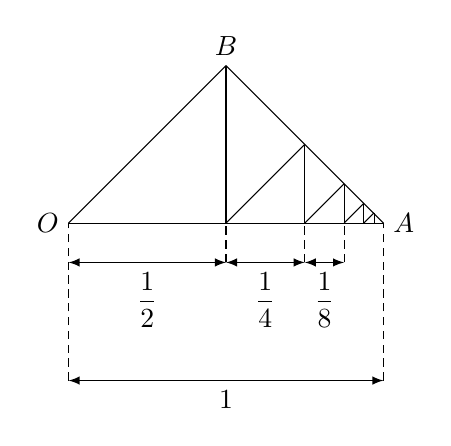
\begin{tikzpicture}[>=latex]
  \draw (0,0) node[left]{$O$}-- (2,2) node[above]{$B$};
  \draw (2,2)-- (2,0);
  \draw (2,2)-- (4,0);
  \draw (2,0)-- (3,1);
  \draw (3,1)-- (3,0);
  \draw (3,0)-- (3.5,0.5);
  \draw (3.5,0.5)-- (3.5,0);
  \draw (3.5,0)-- (3.75,0.25);
  \draw (3.75,0)-- (3.75,0.25);
  \draw (3.75,0)-- (3.88,0.13);
  \draw  (3.88,0.13)-- (3.88,0);
  \draw (0,0) -- (4,0) node[right] {$A$};
  \draw[<->] (0,-0.5) -- (2,-0.5)
     node[midway, below]{$\displaystyle{\frac{1}{2}}$};
  \draw[<->] (2,-0.5) -- (3,-0.5)
     node[midway, below]{$\displaystyle{\frac{1}{4}}$};
  \draw[<->] (3,-0.5) -- (3.5,-0.5)
     node[midway, below]{$\displaystyle{\frac{1}{8}}$};
  \draw[<->] (0,-2) -- (4,-2) node[midway, below]{$1$};
  \draw[densely dashed] (0,-2) -- (0,0) (4,-2) -- (4,0);
  \draw[densely dashed]
    (2,-0.5) -- (2,0) (3,-0.5) -- (3,0) (3.5,-0.5) -- (3.5,0) ;
\end{tikzpicture}

\end{document}
